% LaTeX Article Template
\documentclass[12pt]{article}
%% Other packages
\usepackage{amsmath}
\usepackage{amsthm}
\usepackage{titlesec}
\usepackage{soul}
\usepackage{tikz}
\usepackage{tikz-3dplot}
\usepackage{amssymb}
\usepackage{multicol}
\usepackage{algorithm}
\usepackage{algorithmic}
\usepackage{float}
\usepackage{calc}
\usepackage{fancybox}
\usepackage{array}
\usepackage[shortlabels]{enumitem}
\usepackage{framed}
\usepackage{hyperref}
\newcolumntype{L}[1]{>{\raggedright\let\newline\\\arraybackslash\hspace{0pt}}m{#1}}
\newcolumntype{C}[1]{>{\centering\let\newline\\\arraybackslash\hspace{0pt}}m{#1}}
\newcolumntype{R}[1]{>{\raggedleft\let\newline\\\arraybackslash\hspace{0pt}}m{#1}}


%% Margins
\usepackage{geometry}
\geometry{verbose,letterpaper,tmargin=1in,bmargin=1in,lmargin=1in,rmargin=1in}

\newcommand{\menuchoice}[2]{{\ttfamily#1..#2}}
\newcommand{\dotdot}{..}

\usepackage{graphicx}

% Array vertical and horizontal stretch
% \def\arraystretch{1.5}%  1 is the default, change whatever you need
% \setlength{\tabcolsep}{12pt}

%\graphicspath{%
\graphicspath{{./figs/}}

%% Paragraph style settings
\setlength{\parskip}{\medskipamount}
\setlength{\parindent}{0pt}

%% Change itemize bullets
\renewcommand{\labelitemi}{$\bullet$}
\renewcommand{\labelitemii}{$\circ$}
\renewcommand{\labelitemiii}{$\diamond$}
\renewcommand{\labelitemiv}{$\cdot$}

%% Shrink section fonts
\titleformat*{\section}{\large\bf}
\titleformat*{\subsection}{\normalsize\it}
\titleformat*{\subsubsection}{\normalsize\bf}

% %% Compress the spacing around section titles
\titlespacing*{\section}{0pt}{1.5ex}{0.75ex}
\titlespacing*{\subsection}{0pt}{1ex}{0.5ex}
\titlespacing*{\subsubsection}{0pt}{1ex}{0.5ex}

%% amsthm settings
\theoremstyle{definition}
\newtheorem{problem}{Problem}
\newtheorem{example}{Example}
\newtheorem{mydef}{Definition}

%% Answer box macros
%% \answerbox{alignment}{width}{height}
\newcommand{\answerbox}[3]{%
  \fbox{%
    \begin{minipage}[#1]{#2}
      \hfill\vspace{#3}
    \end{minipage}
  }
}

%% \answerboxfull{alignment}{height}
\newcommand{\answerboxfull}[2]{%
  \answerbox{#1}{\textwidth}{#2} 
}

%% \answerboxone{alignment}{height} -- for first-level bullet
\newcommand{\answerboxone}[2]{%
  \answerbox{#1}{6.15in}{#2} 
}

%% \answerboxtwo{alignment}{height} -- for second-level bullet
\newcommand{\answerboxtwo}[2]{%
  \answerbox{#1}{5.8in}{#2}
}

%% \graphbox{xmin}{xmax}{ymin}{ymax}{scale}
\newcommand{\graphbox}[5]%[-5, 5, -5, 5, 0.33]
{
\begin{tikzpicture}
     [>=latex,scale=#5]
     
     % Coordinate axes
     \draw [->,very thick] (#1, 0) -- (#2, 0) node[right] {$x$};
     \draw [->,very thick] (0, #3) -- (0, #4) node[above] {$y$};
     
     % Grid
     \draw[step=1cm,thick,dotted] (#1,#3) grid (#2,#4);
   \end{tikzpicture}
   }


%% Redefine maketitle
\makeatletter
\renewcommand{\maketitle}{
  \noindent SA403 -- Networks \\

  \begin{center}\Large{\textbf{\@title}}\end{center}
}
\makeatother

% Set the beginning of a LaTeX document
\begin{document}

%\graphbox{-10}{3}{-5}{10}

\title{Lesson 2: Depth and Breadth First Search Algorithms}

%\graphbox[10][10]

\maketitle


\section*{Notes}

Book acknowledgment:
\section*{Goals}
\begin{itemize}
\item Breadth First Search
\item Depth First Search
\end{itemize}

\section{Try it on your own}

Given some graph $G = (V,E)$, how would you systematically explore and number all the connected nodes in $V$?

Try it on this example:

\begin{center}
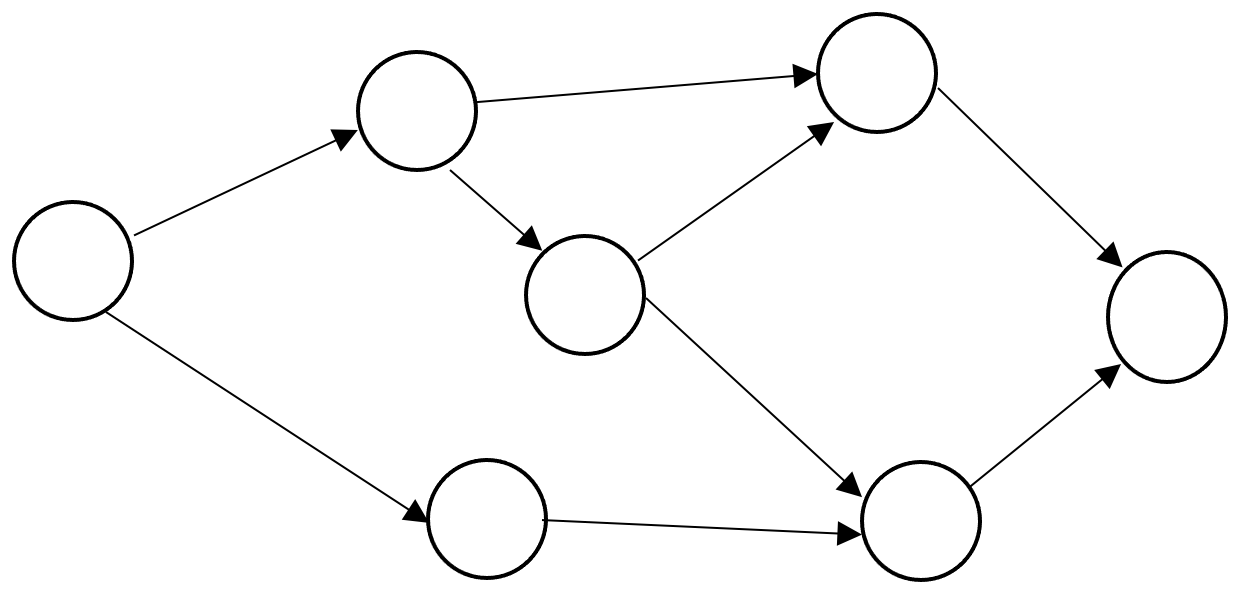
\includegraphics[width=10cm]{searchgraph}
\end{center}

Write down your steps below:
\newpage


\section{Search Algorithms}

Given $s$ as the source node, the two search algorithms we study in this lession will systematically explore the edges of $G$ to \emph{discover} every node that is reachable from $s$. They also calculate the fewest number of edges from $s$ to each reachable node in $G$. While very similar, these two search algorithms differ in implementation and analysis.

\subsection{Breadth First Search}

You can think of the Bread First Search (BFS) algorithm that explores each \emph{layer} of the network

To simplify this algorithm, the BFS signifies each node as \emph{nil}, \emph{discovered}, and \emph{explored}. 

\begin{itemize}
\item All nodes start as nil and may later be explored. 
\item The BFS will keep up with a queue $Q$ that keeps up with the list of nodes that should be explored next.
\end{itemize}


The BFS constructs a BF \emph{\textbf{tree}}, initially containing only its root node $s$. Whenever the search encounters a nil node $v$ in the course of scanning the adjacency list of an already encountered node $u$, the node $v$ and the edge $(u,v)$ are added to the tree. Thus, we refer to the node $u$ as the \textbf{\emph{parent}} of $v$. Since a node is discovered at most once, then each node has at most one parent. 

\emph{\textbf{Written Steps:}}

\vskip .25cm

Initialization: Create queue $Q = \emptyset$. Add source node $s$ to $Q$. Mark $s$ as explored.
\begin{enumerate}
	\item If $Q$ is empty, then proceed to Step \ref{Step3}. Otherwise, remove node $v$ from the bottom of $Q$. Proceed to Step \ref{Step2}. \label{Step1}
	\item For some adjacent node $w \in V$ of $v$, if $w$ is not visited, then add $w$ to the bottom of $Q$, mark $w$ as explored, and set the parent of $w$ to be $v$. Otherwise, repeat Step \ref{Step2}. \label{Step2}
	\item Terminate the algorithm with the BF tree resulting from the parent vector of each node in $V$. \label{Step3}
\end{enumerate}

\emph{\textbf{Pseudocode:}}


\begin{algorithm}
\caption{Determine a BF tree for the Graph $G$ with source node $s$}
\begin{algorithmic} 
%\REQUIRE $n \geq 0 \vee x \neq 0$
%\ENSURE $y = x^n$
\STATE Let $Q$ be the queue
\STATE Add $s$ to $Q$.
\STATE Mark $s$ as explored.
\WHILE{$Q$ is not empty}
	\STATE Remove $v$ from $Q$
	\FOR{all adjacent nodes $w \in \mathcal{V}$ of $v$ }
		\IF{$w$ is not explored}
			\STATE Add $w$ to $Q$
			\STATE Mark $w$ as explored
			\STATE Mark $v$ as the parent of $w$
		\ENDIF
	\ENDFOR

\ENDWHILE
\end{algorithmic}
\end{algorithm}

What do you think are the pros and cons of the BFS algorithm?

\vskip 2cm

Questions?

\vskip 2cm


Run the DFS algorithm on the following graph:

\begin{center}
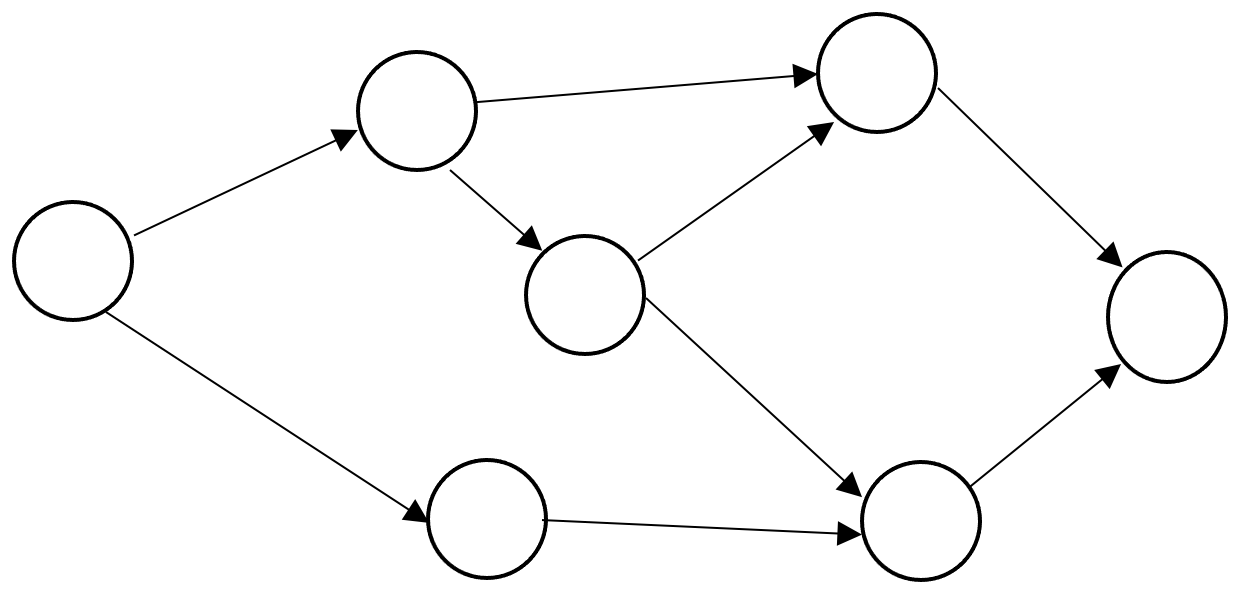
\includegraphics[width=10cm]{searchgraph}
\end{center}



\section{Depth First Search}

Given the name of the Depth First Search (DFS), how do you think it differs from the BFS?

Just like the BFS algorithm, the DFS algorithm also constructs a \emph{\textbf{tree}}, initially containing only its root node $s$. Rather than exploring the \emph{layers} of the graph (as with the BFS algorithm) by exploring \textbf{all} adjacent nodes of each node before moving to another node, the DFS instead continually explores a series of adjacent nodes until the algorithm reaches a node having no adjancent nodes.

The DFS algorithm is a repetitive algorithm that \emph{backtracks} to a recently visited node. 


\emph{\textbf{Written Steps:}}

\vskip .25cm

Initialization: Create stack $S = \emptyset$. Add source node $s$ to the top of $S$. Mark $s$ as explored.
\begin{enumerate}
	\item If $S$ is empty, then proceed to Step \ref{Step3}. Otherwise, remove node $v$ from the top of $S$. Proceed to Step \ref{Step2}. \label{Step1}
	\item For some adjacent node $w \in V$ of $v$, if $w$ is not visited, then add $w$ to the top of $S$, mark $w$ as explored, and set the parent of $w$ to be $v$. Otherwise, repeat Step \ref{Step2}. \label{Step2}
	\item Terminate the algorithm with the DF tree resulting from the parent vector of each node in $V$. \label{Step3}
\end{enumerate}


\emph{\textbf{Pseudocode:}}


\begin{algorithm}
\caption{Determine a DF tree for the Graph $G$ with source node $s$}
\begin{algorithmic} 
\STATE Let $S$ be a stack.
\STATE Insert $s$ at the top of $S$.
\STATE Mark $s$ as explored.
\WHILE{$S$ is not empty}
	\STATE Remove $v$ from the top of $S$
	\FOR{all adjacent nodes $w \in \mathcal{V}$ of $v$ }
		\IF{$w$ is not explored}
			\STATE Add $w$ to the top $Q$
			\STATE Mark $w$ as explored
			\STATE Mark $v$ as the parent of $w$
		\ENDIF
	\ENDFOR

\ENDWHILE
\end{algorithmic}
\end{algorithm}


What do you think are the pros and cons of the BFS algorithm?

\vskip 2cm

Questions?

\vskip 2cm


Run the DFS algorithm on the following graph:

\begin{center}
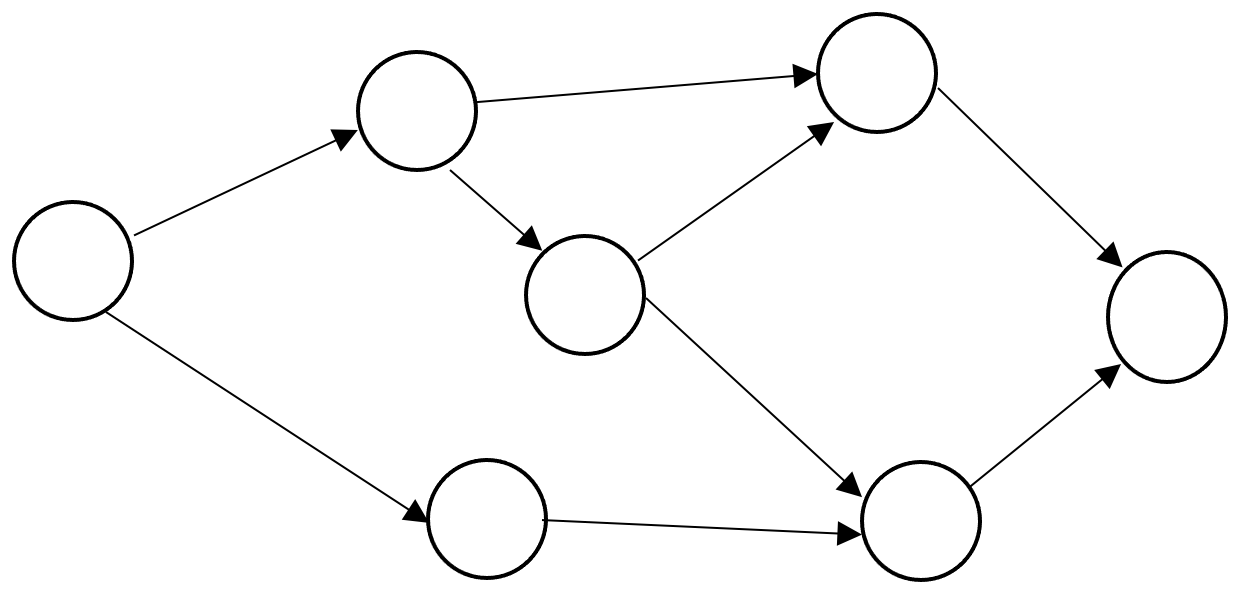
\includegraphics[width=10cm]{searchgraph}
\end{center}



\end{document}
